\section{Introduction}

%Multi-task learning is an inductive learning mechanism to improve generalization performance using related task data.
%Many state-of-the-art results in computer vision and natural language processing are obtained using multi-task learning.
In multi-task learning, having related task data is fundamental to its performance.
Multi-task learning is particularly powerful when there is limited labeled data for a task to be solved, meanwhile more labeled data from different but related tasks is available.
For example, many applications in computer vision \cite{ZSSGM18}, natural language processing \cite{MTDNN19}, and many other areas have been achieved by learning from multiple tasks together.
In spite of these promising empirical results, multi-task learning is not well-understood because of the prevalence of \textit{negative transfer} -- when the trained multi-task model performs worse than single-task learning for the target task.
\todo{transition}
In this work, we present a theoretical study to better understand when multi-task learning works better than single-task learning. % for learning from multiple linear regression tasks.
%We consider a setting where the target task has limited labeled data and show
%On the other hand, unless the structures across task data are well-understood, applying multi-task learning on several different datasets often result in suboptimal models (or negative transfer in more technical terms).

\todo{Motivate high-dimensional data.} The technical challenge is to deal with high-dimensional data, in particular when the size of the training set is only a small constant times the feature dimension.
Prior theory is unable to explain a phase transition that occurs when comparing multi-task learning to single-task learning.
In particular in Figure \ref{fig_motivation}, we observe a shift from positive transfer to negative transfer as a parameter of task relatedness.
The theory we develop will provide a precise explanation to such a phenomenon (and more).

To gain insight into the working of multi-task learning, we consider a simplified setting for learning multiple high-dimensional linear regression tasks.
A typical process to do multi-task learning involves two steps:
(i) Jointly learn a shared representation for all the tasks;
(ii) Fine-tune the learnt model on a specific target task.
We focus on a hard parameter sharing model proposed in \cite{WZR20} and identify conditions on when multi-task and transfer learning works, and when it doesn't.
The high-dimensional linear regression setting where the target task data size is limited captures the intuition that the target task only contains limited labeled data.

Concretely, our input consists of $k$ tasks $(X_1, Y_1)$, $(X_2, Y_2)$, $\dots$, $(X_k, Y_k)$.
We shall assume that each task data follows a linear model, i.e. $y_i = X_i \beta_i + \varepsilon_i$, $1\le i\le k$.
Here $\beta_i\in\real^p$ is the model parameter for the $i$-th task.
Each row of $X_i\in\real^{n_i\times p}$ is assumed to be drawn i.i.d. from a fixed distribution with covariance matrix $\Sigma_i$.
We use a shared body $B\in\real^{p\times r}$ for all tasks and a separate prediction head $\set{W_i \in \real^{r}}_{i=1}^k$ for each task.
%    \paragraph{Different covariates:}
This corresponds to minimizing the following optimization objective.
\begin{align}
	\label{eq_mtl}
	f(B; W_1, \dots, W_k) = \sum_{i=1}^k \norm{X_i B W_i - Y_i}^2.
\end{align}
Note that we consider the natural parameterization without reweighting the tasks above.
The shared body $B$ plays an important role because it allows information transfer between different task data.
This is known as the hard parameter sharing architecture in the literature, where we control the capacity $r$ of $B$, e.g. \cite{KD12,WZR20}.

\begin{figure}[!t]
	\centering
	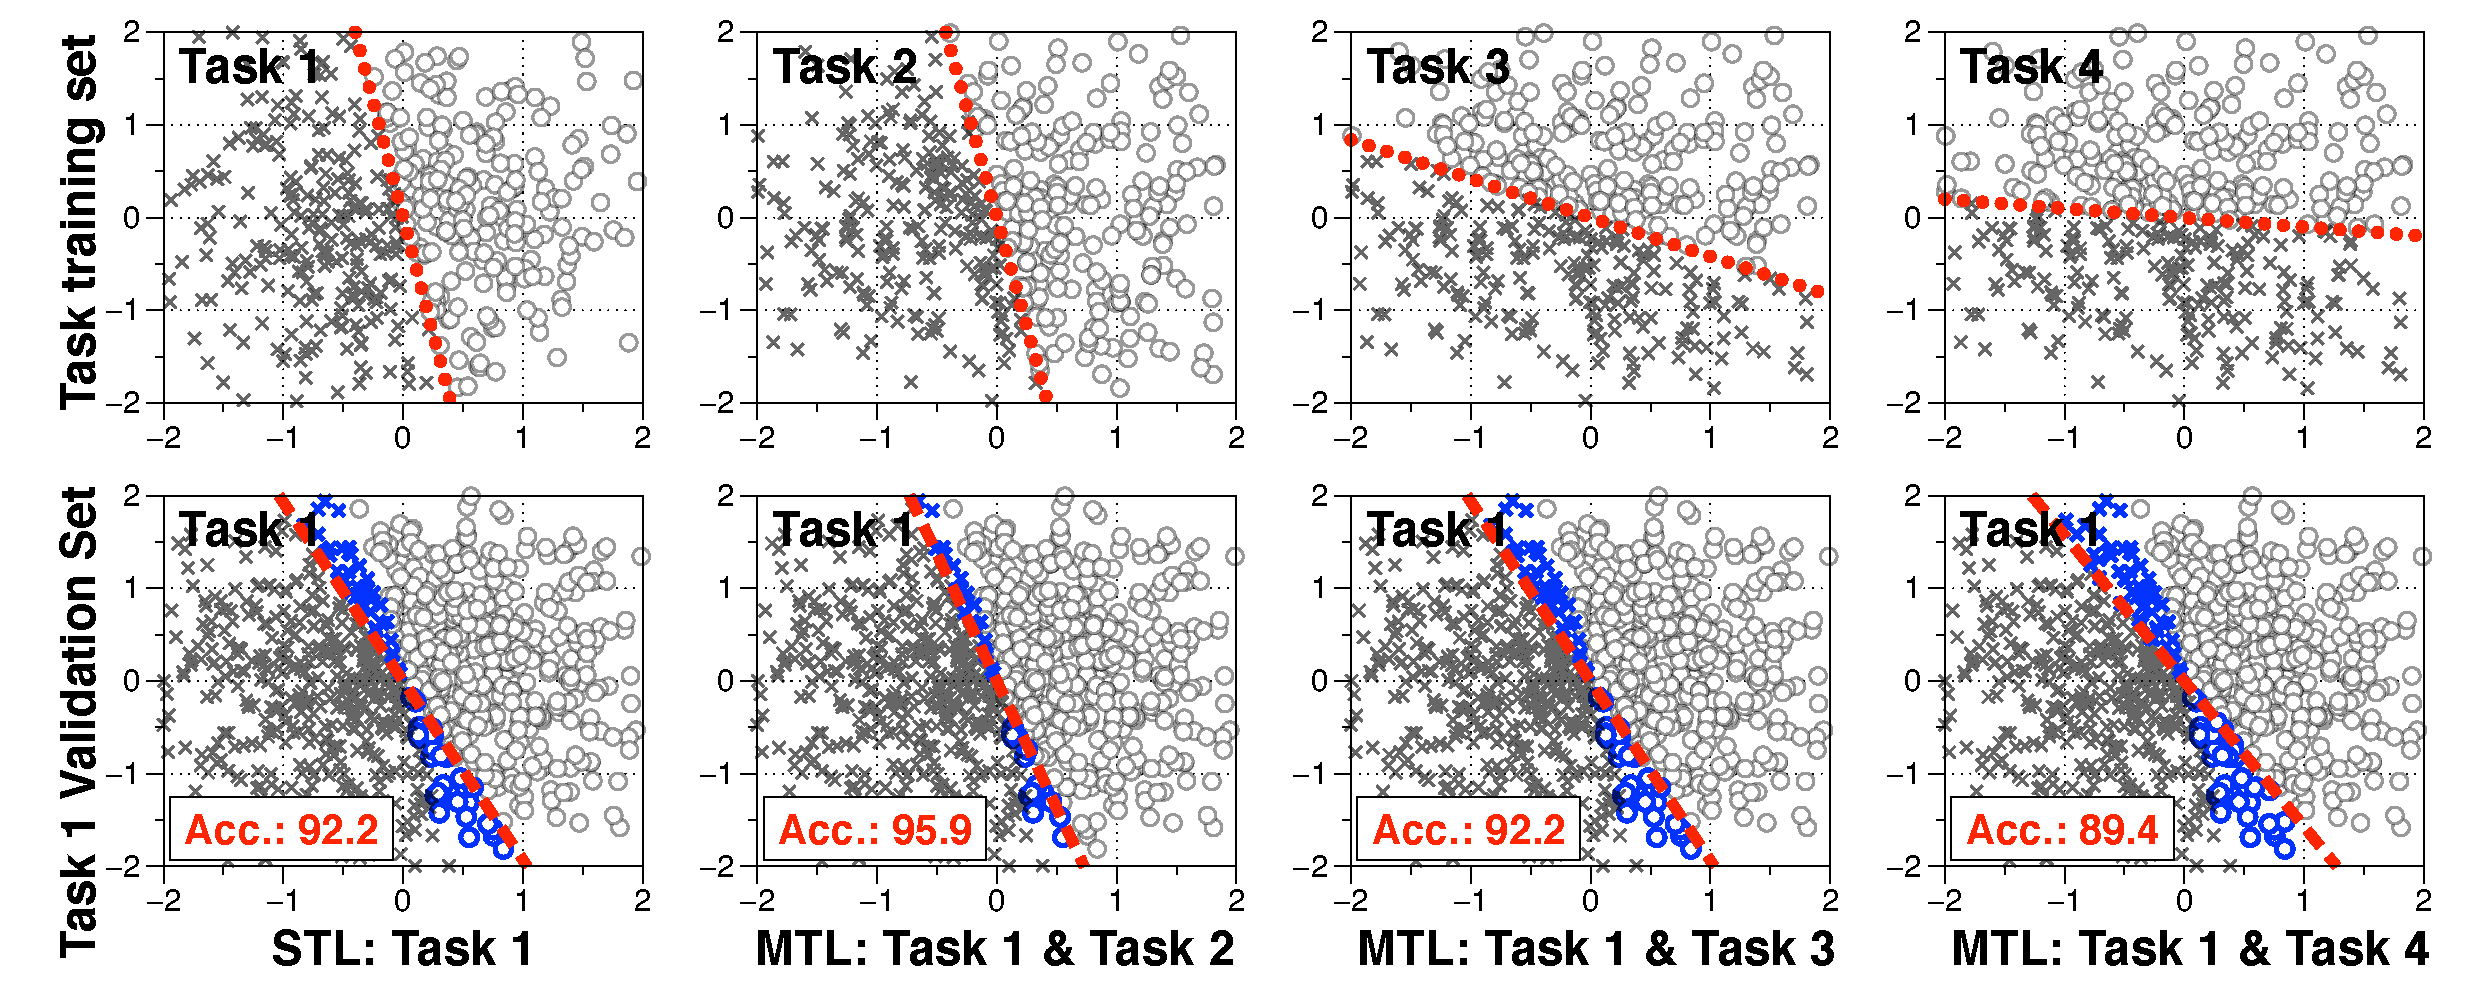
\includegraphics[width=0.8\textwidth]{figures/model_distance_motivation.pdf}
	\caption{Phase transition as a parameter of model distance.}
	\label{fig_motivation}
\end{figure}

We focus on comparing the test performance on a target task using estimators from doing multi-task training and transfer learning.
We compare the test performance of these estimators to the single-task baseline.
The details are described in Algorithm \ref{alg_estimator}.

%We formulate the heterogeneity between different task data under covariate and model shifts .
By using random matrix theory, we can explain several phenomena that are not explained by the techniques of \cite{WZR20}.
\todo{list those here}
We refine the task covariance part of \cite{WZR20} into three factors: model distance, covariate shift matrix and data ratio \cite{PY09,K18}.
These are achieved through tight generalization bounds established in the high-dimensional regression setting.
Our main results are described as follows.

\begin{algorithm}[!t]
	\caption{Multi-task learning using a hard-parameter sharing architecture}
	\label{alg_estimator}
	\begin{algorithmic}[1]
		\Input Two regression tasks $(X_1, Y_2)$, $(X_2, Y_2)$.
		\Param Shared body $B$, task-specific prediction heads $W_1, W_2$.
		\State Training the shared body $B$.
		\State Optimizing the task heads on the validation set

		\begin{itemize}
			\item Jointly optimizing both tasks: $\hat{\beta}_t^{\MTL}$
			\item Optimizing the target task: $\hat{\beta}_t^{\TL}$
			\item Single-task training baseline: $\hat{\beta}_t^{\STL}$
		\end{itemize}
		\State Problem statement: how can we compare the test error of the three estimators on the target task?
		%, $\te(\hat{\beta}_t^{\MTL})$, $\te(\hat{\beta}_t^{\STL})$ and $\te(\hat{\beta}_t^{\TL})$?
	\end{algorithmic}
\end{algorithm}

\smallskip
\noindent{\bf Variance reduction from information transfer.}
	We show that the benefit from doing multi-task or transfer learning stems from reducing the variance of the estimator for the target task through newly added source task data.
	We derive this result for the setting of two tasks with general inputs and $k$ tasks with the same covariates for any $k \ge 2$.
	The latter setting is prevalent in applications of multi-task learning to image classification, where there are multiple prediction labels/tasks for every image \cite{EA20}.
%	First, we provide a precise analysis for performing multi-task learning over two tasks under covariate and model shifts.
	On the other hand, the difference between task models causes a negative effect that we call the \textit{model shift bias}.
	We show bounds on the trade-off between the amount of variance reduced and the amount of model shift bias incurred, which become tighter and tighter as the number of source task data points increases.

	{\it Insight 1}: $\hat{\beta}_t^{\MTL}$ vs $\hat{\beta}_t^{\STL}$.
	With multi-task training, since the training objective balances the losses from both the source and target tasks, the trained model can have worse performance for the target task.
	In particular, if model shift is too large, we get negative transfer from multi-task training.

	{\it Insight 2}: $\hat{\beta}_t^{\TL}$ vs $\hat{\beta}_t^{\MTL}$.
	Finally, we show that the transfer learning estimator always improves over mutli-task training.
	The amount of improvement becomes more significant as the model distance becomes larger.

%	We show the result for two settings: 2 tasks with different covariates, and $k$ tasks that all share the same covariates.
%	We show that our results and insights from the above can be extended to this setting as well.
	%{\bf Negative transfer from model shift:} To complement the above result, we establish a fundamental limit of multi-task learning compared to single-task learning in the presence of model shift.
	%The phenomenon of negative transfer persists despite changing the model capacity or reweighting the tasks. [\textbf{done}]

%\noindent{\bf Variance reduction from information transfer.}
%	Second, we apply our general theory to compare the performance of three different estimators for the target task: multi-task training, single-task training and transfer learning.
%	\begin{enumerate}

\smallskip
	\noindent\textbf{Covariate shift and data ratio.}
	For the case of two tasks with general inputs, we further study the factors that determine the transfer rate.
	We identify two factors, the covariate shift matrix and the ratio between number of task data.
%	Next we show that if we we only optimize the multi-task model on the target task, then we always obtain improved performance over single-task training.
%	We provide fine-grained understanding on the amount of improvement that depends on covariate shift and data ratio.

	\textit{Insight 3}: $\hat{\beta}_t^{\TL}$ vs $\hat{\beta}_t^{\STL}$.
	Our result has implications on the following question.
	Is it better for two tasks to have the same covariance matrix or complementary covariance matrices.
	For our setting, we show that when the data ratio is large, having the same covariance matrix provably yields the lowest test performance on the target task.
	On the other hand, when data ratio is small, we find that there are cases when having complementary covariance matrices is better.
	The result provides insight into why the covariance alignment algorithm can help improve performance in \cite{WZR20}.

\smallskip
	\noindent\textbf{Experimental results.}


